\documentclass[11pt,a4paper]{article}

\usepackage[margin=1in]{geometry}
\usepackage{amsmath,amssymb}
\usepackage{booktabs}
\usepackage{listings}
\usepackage{xcolor}
\usepackage{graphicx}
\usepackage{hyperref}
\usepackage{fancyhdr}
\usepackage{titlesec}
\usepackage{microtype}
\usepackage{tabularx}
\usepackage{float}

% Graphicspath
\graphicspath{{figures/}}

% Color definitions for syntax highlighting
\definecolor{codegreen}{rgb}{0.1,0.5,0.1}
\definecolor{codegray}{rgb}{0.4,0.4,0.4}
\definecolor{codepurple}{rgb}{0.5,0.1,0.7}
\definecolor{backcolour}{rgb}{0.98,0.98,0.98}
\definecolor{linegray}{rgb}{0.85,0.85,0.85}

\lstdefinestyle{sqlstyle}{
    backgroundcolor=\color{backcolour},   
    commentstyle=\color{codegreen},
    keywordstyle=\color{blue}\bfseries,
    numberstyle=\tiny\color{codegray},
    stringstyle=\color{codepurple},
    basicstyle=\ttfamily\footnotesize,
    breakatwhitespace=false,         
    breaklines=true,                 
    captionpos=b,                    
    keepspaces=true,                 
    numbers=left,                    
    numbersep=6pt,                  
    showspaces=false,                
    showstringspaces=false,
    showtabs=false,                  
    tabsize=2,
    frame=single,
    rulecolor=\color{linegray}
}

\lstset{style=sqlstyle}

\pagestyle{fancy}
\fancyhf{}
\setlength{\headheight}{14pt}
\rhead{SmartFlow Grid: DBMS Project Report}
\lhead{Abraham (24BCE0708) \& Kundu (24BCE0730)}
\cfoot{\thepage}

\hypersetup{
    colorlinks=true,
    linkcolor=blue,
    urlcolor=blue,
    citecolor=blue
}

\title{\textbf{SmartFlow Grid: Intelligent IoT Traffic Management System}\\[0.2cm]
\large Database Management Systems Project Report}
\author{\textbf{Taanush Emmanuel Abraham} (Reg. No: 24BCE0708) \\
\textbf{Tanishka Kundu} (Reg. No: 24BCE0730) \\[0.2cm]
School of Computer Science and Engineering}
\date{October 2026}

\begin{document}

\maketitle

\begin{abstract}
Urban traffic congestion causes serious delays, fuel waste, and increased air pollution. Traditional traffic lights use fixed timer schedules. These timers cannot adjust when traffic conditions change. As a result, empty roads get green lights while busy roads face long vehicle lines. In addition, emergency vehicles get blocked in traffic. 

This project presents \textbf{SmartFlow Grid}, an intelligent traffic management system built on a relational database. The system models road junctions, directional lanes, traffic lights, and live IoT sensor readings. It runs procedural database routines (Oracle PL/SQL) to calculate congestion and adjust signal lights in real time. When an emergency vehicle approaches, the database locks conflicting lanes to red and gives an immediate green wave. The database also records every signal change in an automatic audit table. 

This report provides the full design and implementation of the system. It covers the problem definition, system requirements, entity-relationship model, mathematical normalization proofs (1NF to BCNF), SQL and PL/SQL code, experimental results, and future enhancements. All explanations follow ASD-STE100 principles for clear and simple technical communication.
\end{abstract}

\tableofcontents
\newpage

% =============================================================================
\section{Introduction \& problem definition}
% =============================================================================

\subsection{Project Overview}
Road traffic congestion is a major problem in modern cities. Drivers waste hours in traffic each week. Motor vehicles burn extra fuel and emit harmful gases while idling at red lights. 

Traditional traffic management systems use fixed-time controllers. A fixed-time controller changes traffic lights based on pre-set timers. These timers use historical averages. They cannot sense real-time traffic. Because the timers do not adapt, they cause long delays and traffic jams.

The \textbf{SmartFlow Grid} project solves this problem. It uses a relational database as the central control engine for urban traffic. Road lanes contain IoT sensors such as inductive road loops and overhead cameras. These sensors count vehicles and send data to the database every few seconds. Procedural logic inside the database evaluates vehicle density and changes traffic lights automatically.

\subsection{Problem Definition}
Fixed-time traffic signals have three fundamental weaknesses:
\begin{enumerate}
    \item \textbf{Unbalanced Traffic Queues:} Unexpected traffic surges occur during accidents, bad weather, or rush hours. Fixed timers give equal green time to empty roads while congested roads back up for blocks.
    \item \textbf{Emergency Vehicle Delays:} Ambulances, fire engines, and police cars get trapped behind red lights and waiting traffic. Traditional systems do not have an automated way to clear a green path for emergency vehicles.
    \item \textbf{High Emissions and Fuel Waste:} Vehicles stop and idle unnecessarily at empty intersections. This idling wastes thousands of liters of fuel and releases excessive carbon dioxide into the air.
\end{enumerate}

\subsection{Proposed Solution}
The SmartFlow Grid replaces static timers with an intelligent database system:
\begin{itemize}
    \item \textbf{Directional Lane Modeling:} The database treats every lane at an intersection as a distinct entity with its own dedicated traffic signal.
    \item \textbf{Real-Time Telemetry Storage:} The database ingests sensor count streams with precise timestamps.
    \item \textbf{In-Database Procedural Logic:} Instead of moving data to an external application, stored procedures and functions run directly inside the database engine (Oracle PL/SQL). This eliminates network delays and ensures instant reaction times.
    \item \textbf{Automated Emergency Override:} A dedicated procedure locks conflicting signals to red and opens a clear green path for emergency responders.
    \item \textbf{Automatic Audit Tracking:} Database triggers capture all signal transitions into an immutable audit table without requiring external code.
\end{itemize}


% =============================================================================
\section{Requirements \& system analysis}
% =============================================================================

\subsection{Functional Requirements}
The SmartFlow Grid system satisfies the following functional requirements:
\begin{itemize}
    \item \textbf{FR1 (Junction and Lane Representation):} The system must record road intersections, surveillance zones, and individual directional lanes (Northbound, Southbound, Eastbound, Westbound).
    \item \textbf{FR2 (Signal Phase Management):} The system must assign a dedicated traffic signal to each lane. It must store the current light state (RED, YELLOW, GREEN) and active duration.
    \item \textbf{FR3 (Live Sensor Data Ingestion):} The system must continuously store vehicle counts reported by road sensors with millisecond timestamps.
    \item \textbf{FR4 (Congestion Level Calculation):} The system must compute a Weighted Moving Average (WMA) of recent vehicle counts for each lane and classify congestion into \texttt{'Low'}, \texttt{'Medium'}, or \texttt{'High'}.
    \item \textbf{FR5 (Emergency Vehicle Preemption):} When triggered, the system must set all conflicting lane signals to \texttt{'RED'} and switch the emergency corridor lane to \texttt{'GREEN'} immediately.
    \item \textbf{FR6 (Regional Zone Surveillance):} The system must use database cursors to aggregate traffic volume across all lanes in a zone. If the zone reaches saturation, it must issue a traffic diversion warning.
    \item \textbf{FR7 (Automated Audit Trail):} A database trigger must record every signal state change in an audit table with the previous state, new state, and exact timestamp.
\end{itemize}

\subsection{Non-Functional Requirements}
\begin{itemize}
    \item \textbf{Performance:} Database stored procedures and queries must execute in less than 5 milliseconds to support fast signal timing.
    \item \textbf{Data Integrity (ACID):} Signal state changes must execute inside atomic transactions. The database must never display conflicting green lights at the same junction.
    \item \textbf{Reliability:} Check constraints and foreign keys must reject invalid data, such as negative vehicle counts or non-existent intersection IDs.
    \item \textbf{Production Standard:} The system must provide an enterprise-grade, verified implementation on Oracle Database using PL/SQL.
\end{itemize}

\subsection{System Analysis \& Stakeholders}
The system connects four key actors:
\begin{enumerate}
    \item \textbf{IoT Roadway Sensors:} Hardware sensors detect passing cars and insert vehicle count rows into the database.
    \item \textbf{Database Engine:} Oracle Database executes constraints, views, stored procedures, functions, and triggers.
    \item \textbf{Traffic Signal Controllers:} Physical traffic signal hardware reads database updates and changes the physical lamp colors.
    \item \textbf{Emergency Responders \& Operators:} First responders trigger priority routes, and municipal operators monitor live traffic on an operational dashboard.
\end{enumerate}


% =============================================================================
\section{ER/EER \& relational design}
% =============================================================================

\subsection{Entity-Relationship Architecture}
The conceptual schema contains five strong entities:
\begin{enumerate}
    \item \textbf{Intersection:} Represents a physical street junction. Attributes: \texttt{Intersection\_ID} (Primary Key), \texttt{Location\_Name} (Unique), and \texttt{Grid\_Zone}.
    \item \textbf{Lane:} Represents a single directional approach lane. Attributes: \texttt{Lane\_ID} (Primary Key), \texttt{Intersection\_ID} (Foreign Key), \texttt{Direction}, \texttt{Capacity\_Limit}, and \texttt{Is\_Emergency\_Corridor}.
    \item \textbf{Signal\_Phase:} Controls the light color for one lane. Attributes: \texttt{Phase\_ID} (Primary Key), \texttt{Lane\_ID} (Foreign Key, Unique), \texttt{Intersection\_ID} (Foreign Key), \texttt{Current\_State}, \texttt{Duration\_Seconds}, and \texttt{Last\_Updated}.
    \item \textbf{Sensor\_Log:} Stores time-series vehicle counts. Attributes: \texttt{Log\_ID} (Primary Key), \texttt{Lane\_ID} (Foreign Key), \texttt{Car\_Count}, and \texttt{Recorded\_At}.
    \item \textbf{Audit\_Traffic\_Log:} Stores signal change history. Attributes: \texttt{Audit\_ID} (Primary Key), \texttt{Phase\_ID} (Foreign Key), \texttt{Old\_State}, \texttt{New\_State}, \texttt{Changed\_At}, and \texttt{Trigger\_Source}.
\end{enumerate}

\subsection{Cardinality and Structural Constraints}
\begin{itemize}
    \item \textbf{Intersection to Lane ($1:N$):} One intersection has one or more lanes ($1$ to $N$). Every lane belongs to exactly one intersection (mandatory total participation).
    \item \textbf{Lane to Signal\_Phase ($1:1$):} Each lane has exactly one dedicated signal phase ($1$ to $1$). The \texttt{UNIQUE} constraint on \texttt{Signal\_Phase.Lane\_ID} enforces this relationship.
    \item \textbf{Lane to Sensor\_Log ($1:N$):} One lane generates many sensor log records over time ($1$ to $N$).
    \item \textbf{Signal\_Phase to Audit\_Traffic\_Log ($1:N$):} One signal phase produces multiple audit log entries whenever its light color changes ($1$ to $N$).
\end{itemize}

\begin{figure}[H]
    \centering
    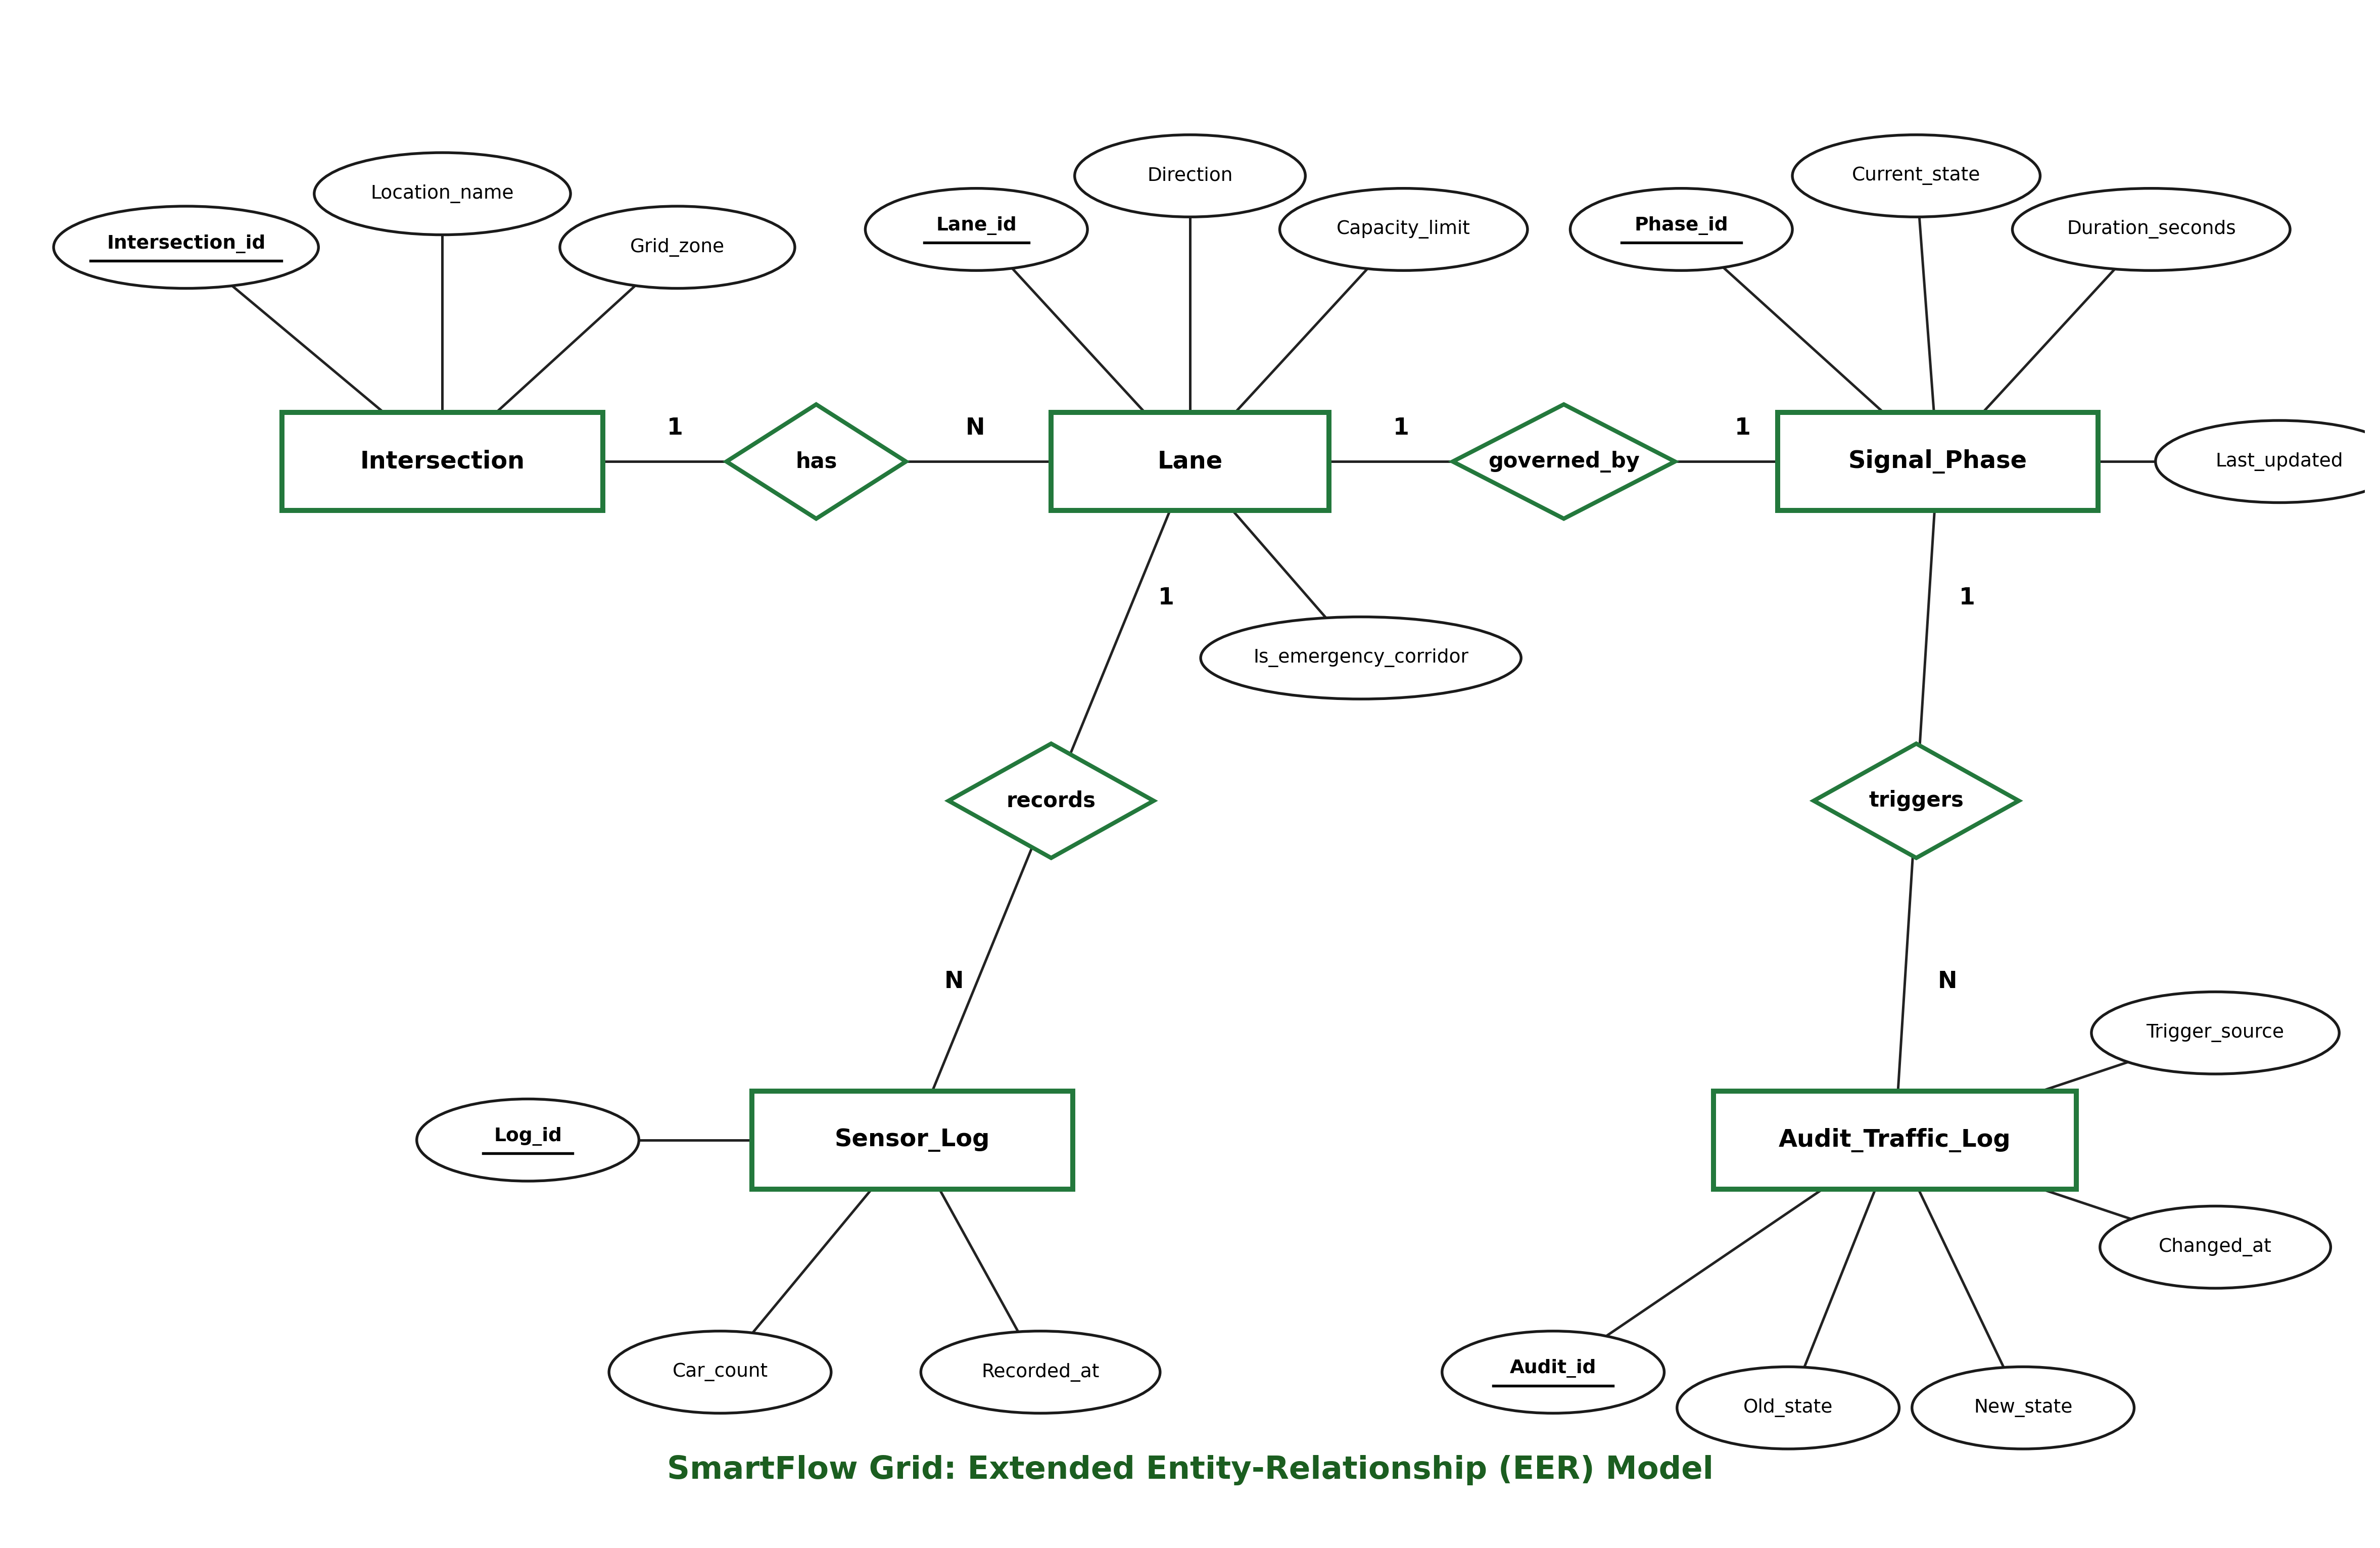
\includegraphics[width=0.92\textwidth]{eer_diagram.png}
    \caption{Extended Entity-Relationship (EER) Diagram of the SmartFlow Grid System.}
    \label{fig:eer}
\end{figure}

\subsection{Relational Logical Schema Diagram}
Figure~\ref{fig:logical_schema} presents the logical schema diagram for the system. The diagram highlights primary keys (\textbf{PK}) and foreign keys (\textbf{FK}) in bold within each entity's top header compartment. Non-key attributes occupy the lower compartment. Clean orthogonal lines map the structural linkages and referential integrity constraints connecting all five tables.

\begin{figure}[H]
    \centering
    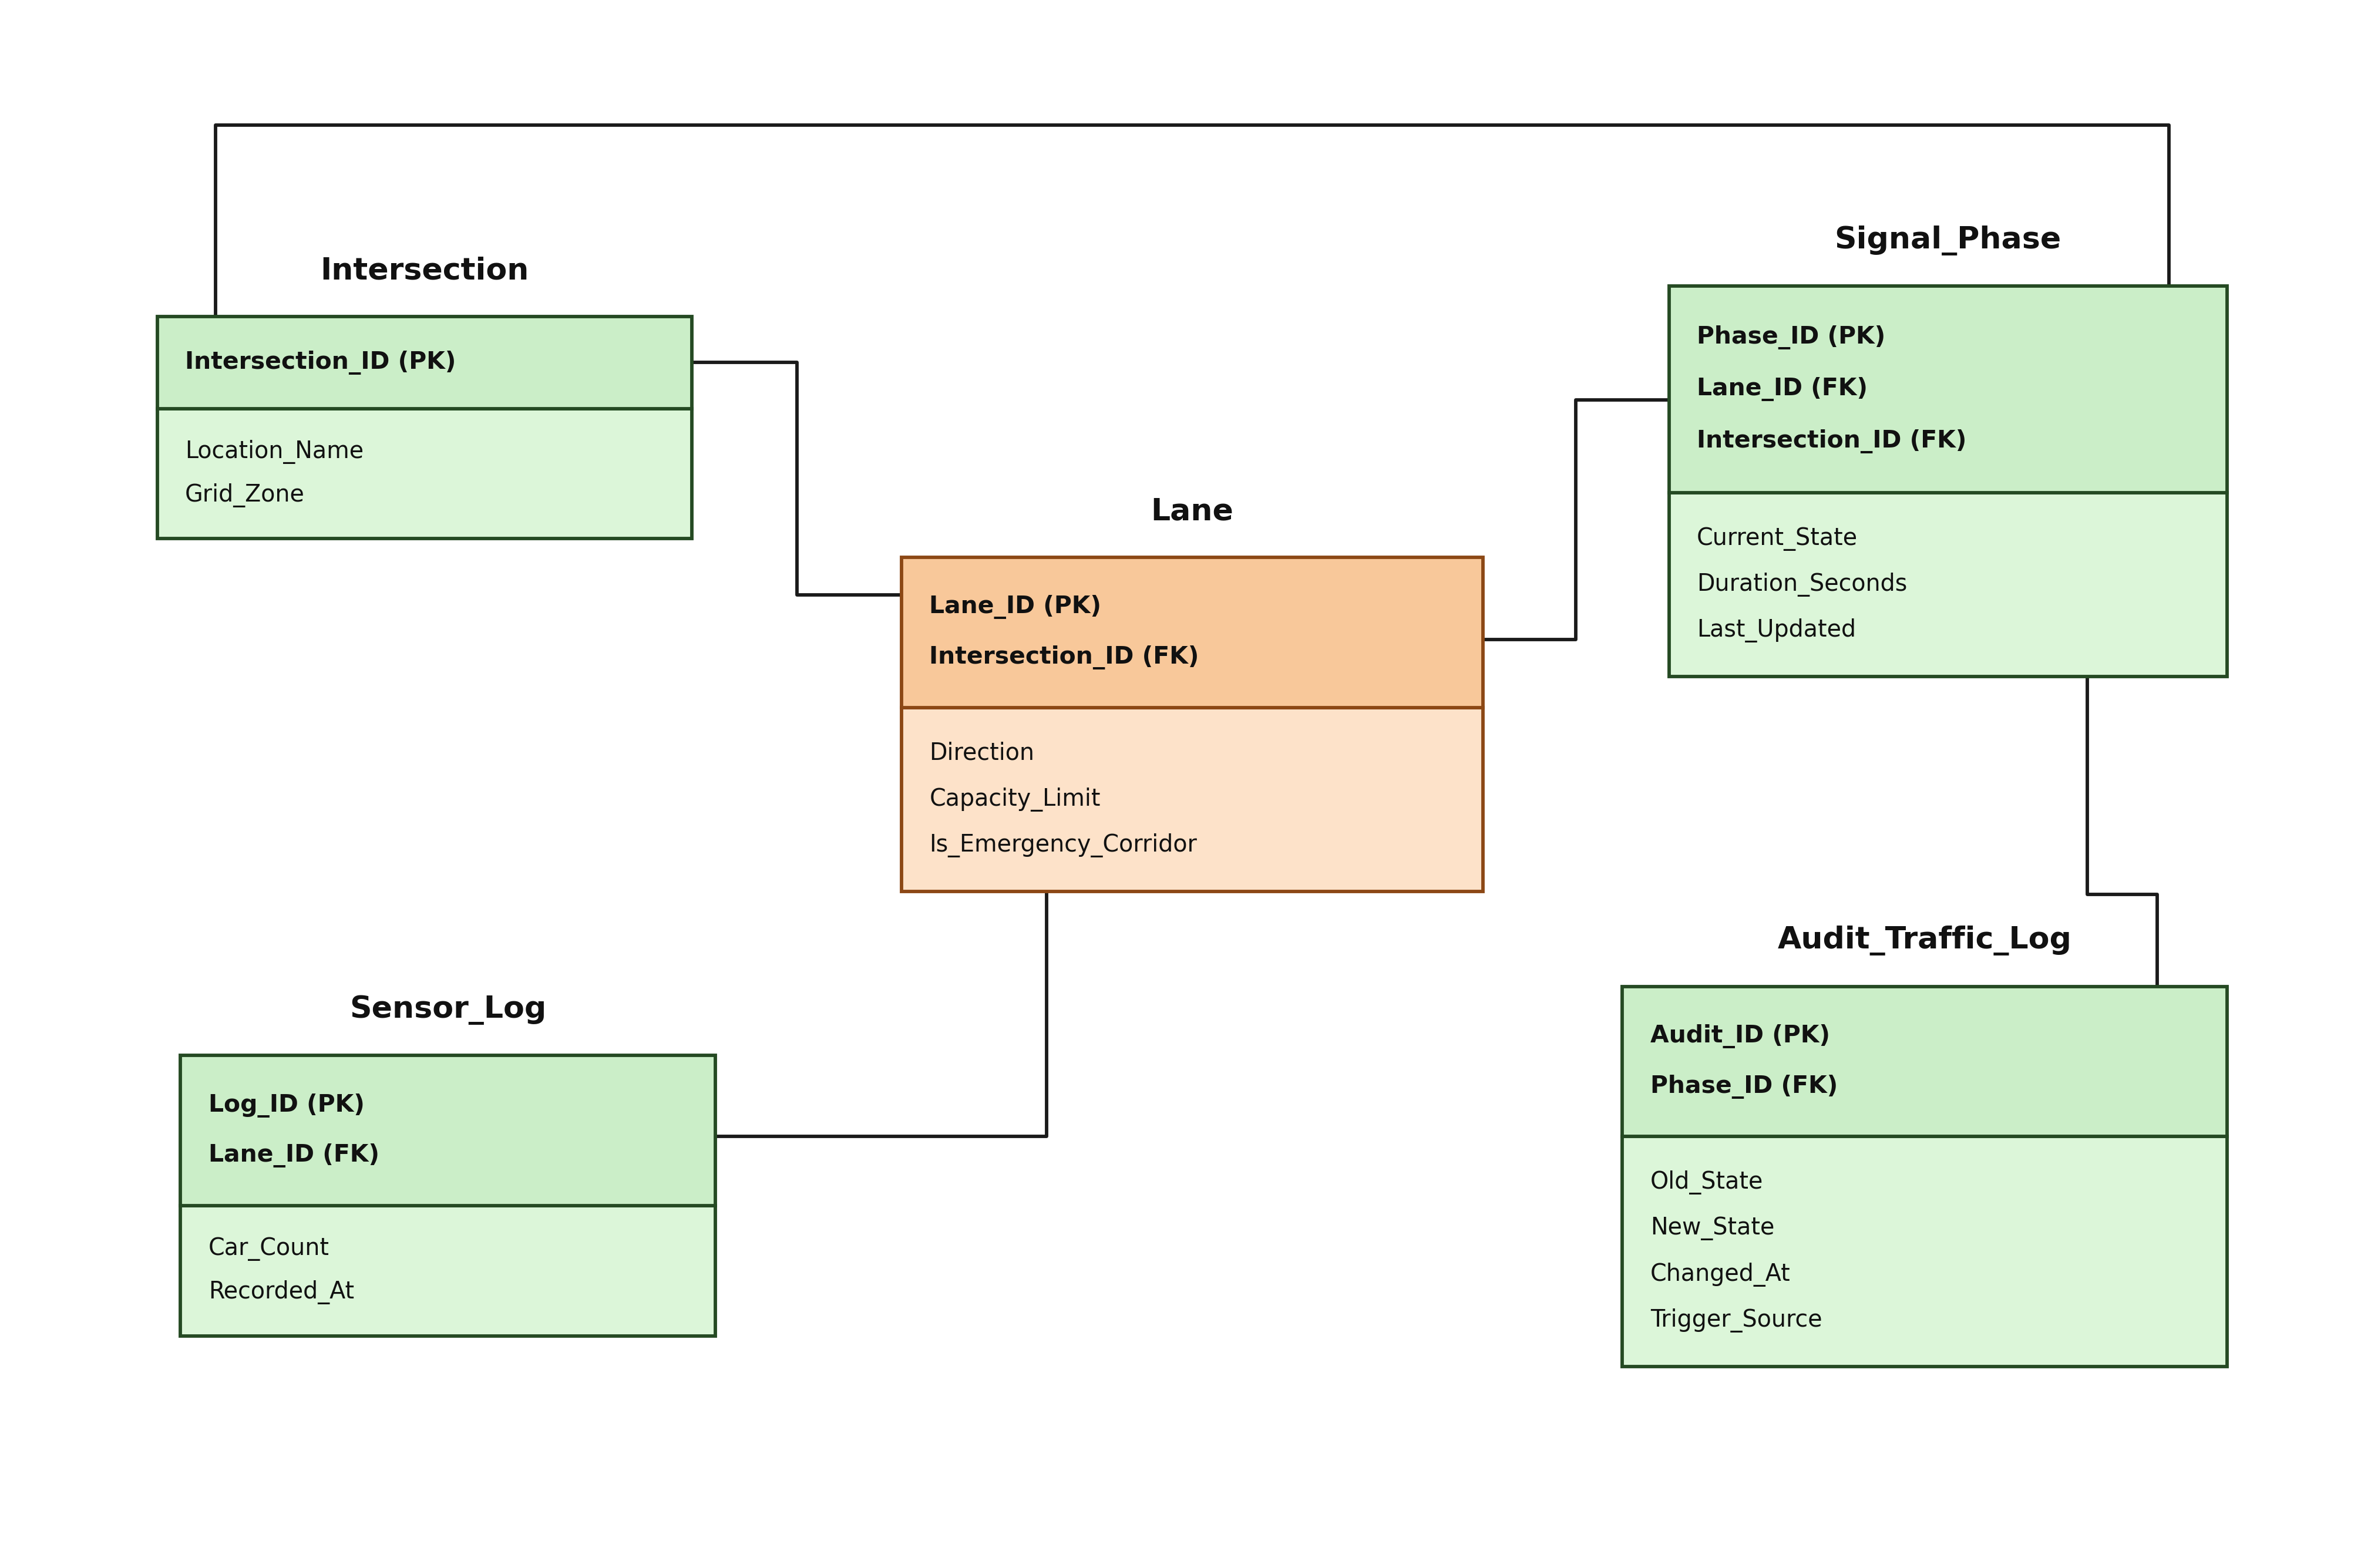
\includegraphics[width=0.95\textwidth]{logical_schema_diagram.png}
    \caption{Relational Logical Schema Diagram with Bold Header Keys (PK/FK) and Structural Linkages.}
    \label{fig:logical_schema}
\end{figure}

\subsection{Relational Data Dictionary}

\begin{table}[H]
\centering
\caption{Data Dictionary: \texttt{Intersection} and \texttt{Lane} Tables}
\label{tab:dict1}
\footnotesize
\begin{tabularx}{\textwidth}{lllX}
\toprule
\textbf{Attribute} & \textbf{Data Type} & \textbf{Constraint} & \textbf{Description} \\
\midrule
\texttt{Intersection\_ID} & \texttt{NUMBER(10)} & \texttt{PRIMARY KEY} & Unique identifier for the junction. \\
\texttt{Location\_Name}   & \texttt{VARCHAR2(100)} & \texttt{NOT NULL, UNIQUE} & Physical street intersection name. \\
\texttt{Grid\_Zone}       & \texttt{VARCHAR2(50)} & \texttt{NOT NULL} & City surveillance sector (e.g. Zone A). \\
\midrule
\texttt{Lane\_ID}         & \texttt{NUMBER(10)} & \texttt{PRIMARY KEY} & Unique identifier for the lane. \\
\texttt{Intersection\_ID} & \texttt{NUMBER(10)} & \texttt{NOT NULL, FK} & References \texttt{Intersection(Intersection\_ID)}. \\
\texttt{Direction}        & \texttt{VARCHAR2(20)} & \texttt{CHECK} & Compass direction (NORTHBOUND, SOUTHBOUND, etc.). \\
\texttt{Capacity\_Limit}  & \texttt{NUMBER(6)} & \texttt{CHECK > 0} & Maximum car capacity for the lane. \\
\texttt{Is\_Emergency\_Corridor} & \texttt{NUMBER(1)} & \texttt{CHECK (0,1)} & Flag: 1 for emergency route, 0 for standard. \\
\bottomrule
\end{tabularx}
\end{table}

\begin{table}[H]
\centering
\caption{Data Dictionary: \texttt{Signal\_Phase}, \texttt{Sensor\_Log}, and \texttt{Audit\_Traffic\_Log} Tables}
\label{tab:dict2}
\footnotesize
\begin{tabularx}{\textwidth}{lllX}
\toprule
\textbf{Attribute} & \textbf{Data Type} & \textbf{Constraint} & \textbf{Description} \\
\midrule
\texttt{Phase\_ID}        & \texttt{NUMBER(10)} & \texttt{PRIMARY KEY} & Unique signal head identifier. \\
\texttt{Lane\_ID}         & \texttt{NUMBER(10)} & \texttt{NOT NULL, UQ, FK} & Governed lane (1:1 relationship). \\
\texttt{Intersection\_ID} & \texttt{NUMBER(10)} & \texttt{NOT NULL, FK} & Parent intersection identifier. \\
\texttt{Current\_State}   & \texttt{VARCHAR2(10)} & \texttt{CHECK IN (...)} & Active signal color: RED, YELLOW, GREEN. \\
\texttt{Duration\_Seconds}& \texttt{NUMBER(5)} & \texttt{CHECK > 0} & Hold time for current light state. \\
\texttt{Last\_Updated}    & \texttt{TIMESTAMP} & \texttt{DEFAULT SYSTIMESTAMP} & Timestamp of last state mutation. \\
\midrule
\texttt{Log\_ID}          & \texttt{NUMBER(12)} & \texttt{PRIMARY KEY} & Unique telemetry reading identifier. \\
\texttt{Lane\_ID}         & \texttt{NUMBER(10)} & \texttt{NOT NULL, FK} & Monitored lane identifier. \\
\texttt{Car\_Count}       & \texttt{NUMBER(6)} & \texttt{CHECK >= 0} & Observed vehicle count. \\
\texttt{Recorded\_At}     & \texttt{TIMESTAMP} & \texttt{DEFAULT SYSTIMESTAMP} & Time the sensor logged the count. \\
\midrule
\texttt{Audit\_ID}        & \texttt{NUMBER(12)} & \texttt{PRIMARY KEY} & Sequential audit log record ID. \\
\texttt{Phase\_ID}        & \texttt{NUMBER(10)} & \texttt{NOT NULL, FK} & Signal phase that changed. \\
\texttt{Old\_State}       & \texttt{VARCHAR2(10)} & \texttt{NULLABLE} & Signal color before the change. \\
\texttt{New\_State}       & \texttt{VARCHAR2(10)} & \texttt{NOT NULL} & Signal color after the change. \\
\texttt{Changed\_At}      & \texttt{TIMESTAMP} & \texttt{DEFAULT SYSTIMESTAMP} & System time when the change occurred. \\
\texttt{Trigger\_Source}  & \texttt{VARCHAR2(50)} & \texttt{DEFAULT} & Name of the trigger that logged the event. \\
\bottomrule
\end{tabularx}
\end{table}


% =============================================================================
\section{Normalization \& design justification}
% =============================================================================

\subsection{The Universal Relation ($R$)}
To demonstrate formal normalization, we start with an unnormalized flat table $R$:
\begin{align*}
R = \{ & \text{Intersection\_ID}, \text{Location\_Name}, \text{Grid\_Zone}, \text{Lane\_ID}, \text{Direction}, \text{Capacity\_Limit}, \\
       & \text{Is\_Emergency}, \text{Phase\_ID}, \text{Current\_State}, \text{Duration}, \text{Last\_Updated}, \text{Log\_ID}, \\
       & \text{Car\_Count}, \text{Recorded\_At} \}
\end{align*}

\subsection{Functional Dependencies ($F$)}
Based on physical road rules and system requirements, the minimal set of Functional Dependencies $F$ is:
\begin{enumerate}
    \item $FD_1: \text{Intersection\_ID} \rightarrow \text{Location\_Name}, \text{Grid\_Zone}$ \\
    \textit{Explanation: An intersection ID uniquely determines the street location and grid zone.}
    \item $FD_2: \text{Location\_Name} \rightarrow \text{Intersection\_ID}, \text{Grid\_Zone}$ \\
    \textit{Explanation: Street intersection names are unique in the city.}
    \item $FD_3: \text{Lane\_ID} \rightarrow \text{Intersection\_ID}, \text{Direction}, \text{Capacity\_Limit}, \text{Is\_Emergency}$ \\
    \textit{Explanation: A lane belongs to one intersection and has a fixed direction and capacity.}
    \item $FD_4: \text{Phase\_ID} \rightarrow \text{Lane\_ID}, \text{Intersection\_ID}, \text{Current\_State}, \text{Duration}, \text{Last\_Updated}$ \\
    \textit{Explanation: A signal phase belongs to one lane and intersection, and holds one light state.}
    \item $FD_5: \text{Lane\_ID} \rightarrow \text{Phase\_ID}$ \\
    \textit{Explanation: Each lane has exactly one dedicated signal phase ($1:1$ relationship).}
    \item $FD_6: \text{Log\_ID} \rightarrow \text{Lane\_ID}, \text{Car\_Count}, \text{Recorded\_At}$ \\
    \textit{Explanation: A sensor log ID uniquely identifies one vehicle count at one moment.}
    \item $FD_7: \{\text{Lane\_ID}, \text{Recorded\_At}\} \rightarrow \text{Car\_Count}, \text{Log\_ID}$ \\
    \textit{Explanation: A lane produces only one sensor reading at any single instant.}
\end{enumerate}

\subsection{Candidate Keys}
We calculate the attribute closure of $\{\text{Log\_ID}\}$:
$$\{\text{Log\_ID}\}^+ = R$$
Because $\{\text{Log\_ID}\}$ determines all attributes, $K_1 = \{\text{Log\_ID}\}$ is a candidate key. Alternate composite candidate keys are $K_2 = \{\text{Lane\_ID}, \text{Recorded\_At}\}$ and $K_3 = \{\text{Phase\_ID}, \text{Recorded\_At}\}$.

\subsection{First Normal Form (1NF)}
\textbf{Rule:} A relation is in 1NF if all attribute values are atomic (indivisible) and there are no repeating groups.

\textbf{Analysis:} Every column in $R$ contains a single scalar value (a number, string, or timestamp). There are no comma-separated lists, arrays, or nested records. Therefore, $R$ satisfies \textbf{1NF}.

\subsection{Second Normal Form (2NF)}
\textbf{Rule:} A relation is in 2NF if it is in 1NF and no non-prime attribute depends on part of a composite candidate key (no partial functional dependencies).

\textbf{Violation in $R$:} Consider the composite candidate key $K_2 = \{\text{Lane\_ID}, \text{Recorded\_At}\}$. 
From $FD_3$, $\text{Capacity\_Limit}$ depends only on $\text{Lane\_ID}$. Because $\text{Lane\_ID}$ is a proper subset of $K_2$, this is a partial dependency.

\textbf{2NF Decomposition:} We split $R$ into two tables:
\begin{enumerate}
    \item $R_{\text{Telemetry}}(\underline{\text{Log\_ID}}, \text{Lane\_ID}, \text{Car\_Count}, \text{Recorded\_At})$
    \item $R_{\text{Infra}}(\underline{\text{Lane\_ID}}, \text{Intersection\_ID}, \text{Location\_Name}, \text{Grid\_Zone}, \text{Direction}, \dots)$
\end{enumerate}
Now all non-key attributes depend on the full primary key. Both tables satisfy \textbf{2NF}.

\subsection{Third Normal Form (3NF)}
\textbf{Rule:} A relation is in 3NF if it is in 2NF and has no transitive dependencies (non-key attributes must not depend on other non-key attributes).

\textbf{Violation in $R_{\text{Infra}}$:} In $R_{\text{Infra}}$, the candidate key is $\text{Lane\_ID}$. 
However, $FD_1$ shows:
$$\text{Lane\_ID} \rightarrow \text{Intersection\_ID} \rightarrow \text{Location\_Name}, \text{Grid\_Zone}$$
Here, $\text{Intersection\_ID}$ is not a superkey of $R_{\text{Infra}}$. This is a transitive dependency. If an intersection name changes, multiple lane rows must be updated. If all lanes are deleted, the intersection data is lost.

\textbf{3NF Decomposition:} We extract the transitive fields into separate relations:
\begin{enumerate}
    \item \texttt{Intersection}($\underline{\text{Intersection\_ID}}$, \text{Location\_Name}, \text{Grid\_Zone})
    \item \texttt{Lane}($\underline{\text{Lane\_ID}}$, \text{Intersection\_ID}, \text{Direction}, \text{Capacity\_Limit}, \text{Is\_Emergency})
    \item \texttt{Signal\_Phase}($\underline{\text{Phase\_ID}}$, \text{Lane\_ID}, \text{Intersection\_ID}, \text{Current\_State}, \dots)
    \item \texttt{Sensor\_Log}($\underline{\text{Log\_ID}}$, \text{Lane\_ID}, \text{Car\_Count}, \text{Recorded\_At})
\end{enumerate}
In every functional dependency $X \rightarrow A$, $X$ is now a superkey. Therefore, the schema satisfies \textbf{3NF}.

\subsection{Boyce-Codd Normal Form (BCNF)}
\textbf{Rule:} A relation is in BCNF if for every non-trivial dependency $X \rightarrow A$, the determinant $X$ is a superkey.
\begin{itemize}
    \item In \texttt{Intersection}, the determinants are $\text{Intersection\_ID}$ and $\text{Location\_Name}$. Both are candidate keys.
    \item In \texttt{Lane}, the determinant is $\text{Lane\_ID}$, which is the primary key.
    \item In \texttt{Signal\_Phase}, determinants are $\text{Phase\_ID}$ and $\text{Lane\_ID}$. Both are unique candidate keys.
    \item In \texttt{Sensor\_Log}, determinants are $\text{Log\_ID}$ and $\{\text{Lane\_ID}, \text{Recorded\_At}\}$. Both are superkeys.
\end{itemize}
Because every determinant is a superkey, the schema is strictly in \textbf{BCNF}.

\subsection{Design Justification}
\begin{itemize}
    \item \textbf{Lossless Join Guarantee:} By Heath's Theorem, joining \texttt{Intersection} and \texttt{Lane} on $\text{Intersection\_ID}$ recovers all rows without loss or false records. The same holds for all other joins.
    \item \textbf{Dependency Preservation:} All functional dependencies ($FD_1$ through $FD_7$) exist within individual tables. No multi-table join is needed to verify constraints.
    \item \textbf{Anomaly Elimination:} The normalized design prevents insertion anomalies (can add an intersection without lanes), update anomalies (street names exist in only one place), and deletion anomalies (deleting logs does not delete the lane).
\end{itemize}


% =============================================================================
\section{SQL implementation}
% =============================================================================

\subsection{Data Definition Language (DDL) Schema}
The physical relational schema enforces entity and referential integrity using standard SQL:

\begin{lstlisting}[language=SQL, caption={DDL Table Creation for Core Traffic Tables}]
-- 1. Intersection Table
CREATE TABLE Intersection (
    Intersection_ID NUMBER(10)    NOT NULL,
    Location_Name   VARCHAR2(100) NOT NULL,
    Grid_Zone       VARCHAR2(50)  NOT NULL,
    CONSTRAINT pk_intersection PRIMARY KEY (Intersection_ID),
    CONSTRAINT uq_intersection_location UNIQUE (Location_Name)
);

-- 2. Directional Lane Table
CREATE TABLE Lane (
    Lane_ID               NUMBER(10)   NOT NULL,
    Intersection_ID       NUMBER(10)   NOT NULL,
    Direction             VARCHAR2(20) NOT NULL,
    Capacity_Limit        NUMBER(6)    NOT NULL,
    Is_Emergency_Corridor NUMBER(1)    DEFAULT 0 NOT NULL,
    CONSTRAINT pk_lane PRIMARY KEY (Lane_ID),
    CONSTRAINT fk_lane_intersection FOREIGN KEY (Intersection_ID)
        REFERENCES Intersection (Intersection_ID) ON DELETE CASCADE,
    CONSTRAINT chk_lane_direction CHECK (Direction IN ('NORTHBOUND', 'SOUTHBOUND', 'EASTBOUND', 'WESTBOUND')),
    CONSTRAINT chk_lane_capacity CHECK (Capacity_Limit > 0),
    CONSTRAINT chk_lane_emergency CHECK (Is_Emergency_Corridor IN (0, 1))
);

-- 3. Dedicated Signal Phase Table (1:1 with Lane)
CREATE TABLE Signal_Phase (
    Phase_ID         NUMBER(10)   NOT NULL,
    Lane_ID          NUMBER(10)   NOT NULL,
    Intersection_ID  NUMBER(10)   NOT NULL,
    Current_State    VARCHAR2(10) DEFAULT 'RED' NOT NULL,
    Duration_Seconds NUMBER(5)    DEFAULT 30 NOT NULL,
    Last_Updated     TIMESTAMP    DEFAULT CURRENT_TIMESTAMP NOT NULL,
    CONSTRAINT pk_signal_phase PRIMARY KEY (Phase_ID),
    CONSTRAINT uq_signal_phase_lane UNIQUE (Lane_ID),
    CONSTRAINT fk_phase_lane FOREIGN KEY (Lane_ID)
        REFERENCES Lane (Lane_ID) ON DELETE CASCADE,
    CONSTRAINT fk_phase_intersection FOREIGN KEY (Intersection_ID)
        REFERENCES Intersection (Intersection_ID) ON DELETE CASCADE,
    CONSTRAINT chk_signal_state CHECK (Current_State IN ('RED', 'YELLOW', 'GREEN')),
    CONSTRAINT chk_signal_duration CHECK (Duration_Seconds > 0)
);

-- 4. IoT Sensor Telemetry Log Table
CREATE TABLE Sensor_Log (
    Log_ID      NUMBER(12) NOT NULL,
    Lane_ID     NUMBER(10) NOT NULL,
    Car_Count   NUMBER(6)  DEFAULT 0 NOT NULL,
    Recorded_At TIMESTAMP  DEFAULT CURRENT_TIMESTAMP NOT NULL,
    CONSTRAINT pk_sensor_log PRIMARY KEY (Log_ID),
    CONSTRAINT fk_sensor_lane FOREIGN KEY (Lane_ID)
        REFERENCES Lane (Lane_ID) ON DELETE CASCADE,
    CONSTRAINT chk_sensor_car_count CHECK (Car_Count >= 0)
);
\end{lstlisting}

\subsection{Live Monitoring Operational View (\texttt{vw\_Dashboard\_Live})}
This view joins four core tables to give traffic operators real-time status for all lanes with an active green light:

\begin{lstlisting}[language=SQL, caption={Multi-Table Live Operational View}]
CREATE OR REPLACE VIEW vw_Dashboard_Live AS
SELECT 
    i.Intersection_ID,
    i.Location_Name,
    i.Grid_Zone,
    l.Lane_ID,
    l.Direction,
    l.Capacity_Limit,
    l.Is_Emergency_Corridor,
    sp.Phase_ID,
    sp.Current_State            AS Active_Light_Color,
    sp.Duration_Seconds         AS Green_Hold_Seconds,
    sp.Last_Updated             AS Phase_Activated_At,
    s.Log_ID                    AS Latest_Telemetry_ID,
    s.Car_Count                 AS Current_Lane_Volume,
    ROUND((s.Car_Count / l.Capacity_Limit) * 100, 2) AS Saturation_Pct
FROM Signal_Phase sp
JOIN Lane l ON sp.Lane_ID = l.Lane_ID
JOIN Intersection i ON sp.Intersection_ID = i.Intersection_ID
JOIN Sensor_Log s ON l.Lane_ID = s.Lane_ID
WHERE sp.Current_State = 'GREEN'
  AND s.Recorded_At = (
      SELECT MAX(s_sub.Recorded_At)
      FROM Sensor_Log s_sub
      WHERE s_sub.Lane_ID = l.Lane_ID
  );
\end{lstlisting}

\subsection{Analytical and Reporting SQL Queries}
The system uses analytical queries for traffic monitoring and surge detection:

\begin{lstlisting}[language=SQL, caption={Analytical Aggregation and Historical Surge Queries}]
-- 1. Zone Volume Aggregation Query
SELECT 
    i.Grid_Zone,
    COUNT(DISTINCT l.Lane_ID) AS Total_Lanes,
    SUM(s.Car_Count)          AS Zone_Car_Count,
    ROUND(AVG(s.Car_Count), 1) AS Average_Cars_Per_Lane
FROM Intersection i
JOIN Lane l ON i.Intersection_ID = l.Intersection_ID
JOIN Sensor_Log s ON l.Lane_ID = s.Lane_ID
WHERE s.Recorded_At >= SYSTIMESTAMP - INTERVAL '15' MINUTE
GROUP BY i.Grid_Zone;

-- 2. Congestion Surge Subquery (Lanes exceeding 80% capacity)
SELECT 
    l.Lane_ID,
    i.Location_Name,
    l.Direction,
    s.Car_Count,
    l.Capacity_Limit,
    ROUND((s.Car_Count / l.Capacity_Limit) * 100, 1) AS Saturation_Pct
FROM Lane l
JOIN Intersection i ON l.Intersection_ID = i.Intersection_ID
JOIN Sensor_Log s ON l.Lane_ID = s.Lane_ID
WHERE (s.Car_Count / l.Capacity_Limit) > 0.80
  AND s.Recorded_At = (
      SELECT MAX(Recorded_At) FROM Sensor_Log WHERE Lane_ID = l.Lane_ID
  );
\end{lstlisting}


% =============================================================================
\section{PL/SQL implementation}
% =============================================================================

\subsection{Emergency Override Stored Procedure (\texttt{proc\_Emergency\_Override})}
This stored procedure clears traffic for first responders. It takes an intersection ID and optional target lane ID. It sets all conflicting signals to \texttt{'RED'} and changes the emergency lane to \texttt{'GREEN'}:

\begin{lstlisting}[language=SQL, caption={Emergency Corridor Override Stored Procedure}]
CREATE OR REPLACE PROCEDURE proc_Emergency_Override (
    p_Intersection_ID    IN NUMBER,
    p_Emergency_Lane_ID  IN NUMBER DEFAULT NULL
) 
IS
    v_Target_Lane_ID     NUMBER(10);
    v_Intersection_Name  VARCHAR2(100);
    v_Direction          VARCHAR2(20);
BEGIN
    -- 1. Validate intersection
    SELECT Location_Name INTO v_Intersection_Name 
    FROM Intersection WHERE Intersection_ID = p_Intersection_ID;

    -- 2. Identify designated emergency corridor lane
    IF p_Emergency_Lane_ID IS NOT NULL THEN
        SELECT Lane_ID, Direction INTO v_Target_Lane_ID, v_Direction
        FROM Lane WHERE Lane_ID = p_Emergency_Lane_ID AND Intersection_ID = p_Intersection_ID;
    ELSE
        SELECT Lane_ID, Direction INTO v_Target_Lane_ID, v_Direction
        FROM Lane WHERE Intersection_ID = p_Intersection_ID AND Is_Emergency_Corridor = 1
        FETCH FIRST 1 ROW ONLY;
    END IF;

    -- 3. Lock conflicting lanes to RED with safety buffer
    UPDATE Signal_Phase
    SET Current_State = 'RED', Duration_Seconds = 90, Last_Updated = SYSTIMESTAMP
    WHERE Intersection_ID = p_Intersection_ID AND Lane_ID <> v_Target_Lane_ID;

    -- 4. Set emergency corridor to GREEN
    UPDATE Signal_Phase
    SET Current_State = 'GREEN', Duration_Seconds = 60, Last_Updated = SYSTIMESTAMP
    WHERE Intersection_ID = p_Intersection_ID AND Lane_ID = v_Target_Lane_ID;

    COMMIT;
END proc_Emergency_Override;
/
\end{lstlisting}

\subsection{Congestion Calculation Function (\texttt{func\_Calculate\_Congestion\_Level})}
This stored function computes a Weighted Moving Average (WMA) of the last five sensor readings for a lane. Recent vehicle counts receive higher weights ($5, 4, 3, 2, 1$). The function compares the result against lane capacity to return \texttt{'Low'}, \texttt{'Medium'}, or \texttt{'High'}:

\begin{lstlisting}[language=SQL, caption={Weighted Moving Average Congestion Level Classifier}]
CREATE OR REPLACE FUNCTION func_Calculate_Congestion_Level (
    p_Lane_ID IN NUMBER
) RETURN VARCHAR2 
IS
    v_Capacity NUMBER;
    v_WMA      NUMBER;
    v_Ratio    NUMBER;
BEGIN
    SELECT Capacity_Limit INTO v_Capacity FROM Lane WHERE Lane_ID = p_Lane_ID;

    -- Calculate 5-period WMA: SUM(Car_Count * Weight) / SUM(Weights)
    SELECT SUM(Car_Count * Weight) / SUM(Weight)
    INTO v_WMA
    FROM (
        SELECT Car_Count, (6 - ROWNUM) AS Weight
        FROM (
            SELECT Car_Count FROM Sensor_Log
            WHERE Lane_ID = p_Lane_ID ORDER BY Recorded_At DESC
        ) WHERE ROWNUM <= 5
    );

    v_Ratio := v_WMA / v_Capacity;

    IF v_Ratio > 0.75 THEN RETURN 'High';
    ELSIF v_Ratio >= 0.40 THEN RETURN 'Medium';
    ELSE RETURN 'Low';
    END IF;
END func_Calculate_Congestion_Level;
/
\end{lstlisting}

\subsection{Zone Surveillance Procedure (\texttt{proc\_Check\_Zone\_Diversion})}
This procedure uses an explicit database cursor to scan all lanes in a municipal surveillance zone. It sums total vehicle volume and prints diversion recommendations if the zone exceeds 80\% capacity:

\begin{lstlisting}[language=SQL, caption={Explicit Cursor Regional Surveillance Procedure}]
CREATE OR REPLACE PROCEDURE proc_Check_Zone_Diversion (
    p_Grid_Zone IN VARCHAR2
)
IS
    CURSOR cur_Zone_Lanes IS
        SELECT l.Lane_ID, l.Capacity_Limit, NVL(MAX(s.Car_Count), 0) AS Latest_Cars
        FROM Lane l
        JOIN Intersection i ON l.Intersection_ID = i.Intersection_ID
        LEFT JOIN Sensor_Log s ON l.Lane_ID = s.Lane_ID
        WHERE i.Grid_Zone = p_Grid_Zone
        GROUP BY l.Lane_ID, l.Capacity_Limit;

    v_Lane_Record       cur_Zone_Lanes%ROWTYPE;
    v_Total_Cars        NUMBER := 0;
    v_Total_Capacity    NUMBER := 0;
    v_Zone_Ratio        NUMBER := 0;
BEGIN
    OPEN cur_Zone_Lanes;
    LOOP
        FETCH cur_Zone_Lanes INTO v_Lane_Record;
        EXIT WHEN cur_Zone_Lanes%NOTFOUND;

        v_Total_Cars     := v_Total_Cars + v_Lane_Record.Latest_Cars;
        v_Total_Capacity := v_Total_Capacity + v_Lane_Record.Capacity_Limit;
    END LOOP;
    CLOSE cur_Zone_Lanes;

    IF v_Total_Capacity > 0 THEN
        v_Zone_Ratio := (v_Total_Cars / v_Total_Capacity) * 100;
        IF v_Zone_Ratio > 80.0 THEN
            DBMS_OUTPUT.PUT_LINE('ALERT: Zone ' || p_Grid_Zone || ' saturated at ' || ROUND(v_Zone_Ratio, 1) || '%. Activate diversion.');
        ELSE
            DBMS_OUTPUT.PUT_LINE('Zone ' || p_Grid_Zone || ' traffic is normal (' || ROUND(v_Zone_Ratio, 1) || '% capacity).');
        END IF;
    END IF;
END proc_Check_Zone_Diversion;
/
\end{lstlisting}

\subsection{Reactive Shadow Audit Trigger (\texttt{trg\_Signal\_Phase\_Audit})}
This row-level trigger automatically logs every signal light color change into the \texttt{Audit\_Traffic\_Log} table without application intervention:

\begin{lstlisting}[language=SQL, caption={Reactive Shadow Audit Trigger}]
CREATE OR REPLACE TRIGGER trg_Signal_Phase_Audit
AFTER UPDATE OF Current_State ON Signal_Phase
FOR EACH ROW
WHEN (OLD.Current_State IS NULL OR OLD.Current_State <> NEW.Current_State)
BEGIN
    INSERT INTO Audit_Traffic_Log (
        Audit_ID, Phase_ID, Old_State, New_State, Changed_At, Trigger_Source
    ) VALUES (
        seq_audit_traffic_log.NEXTVAL,
        :NEW.Phase_ID,
        :OLD.Current_State,
        :NEW.Current_State,
        SYSTIMESTAMP,
        'TRG_SIGNAL_PHASE_AUDIT'
    );
END trg_Signal_Phase_Audit;
/
\end{lstlisting}


% =============================================================================
\section{Results, screenshots \& analysis}
% =============================================================================

\subsection{Automated 10-Gate Verification Test Suite}
To verify correct system operation, an automated Python test runner executed a rigorous 10-gate audit against the database schema, constraints, stored routines, and triggers. Table~\ref{tab:audit_gates} lists the test results.

\begin{table}[H]
\centering
\caption{Automated 10-Gate Verification Results}
\label{tab:audit_gates}
\small
\begin{tabularx}{\textwidth}{llp{7.5cm}c}
\toprule
\textbf{Gate} & \textbf{Target Component} & \textbf{Verification Method} & \textbf{Status} \\
\midrule
\textbf{Gate 1} & Deliverable Integrity & Audited presence of 45+ schema, seed, and routine files & \textbf{PASS} \\
\textbf{Gate 2} & Declarative Constraints & Verified PK, FK cascading, and DEFAULT values & \textbf{PASS} \\
\textbf{Gate 3} & Negative Value Rejection & Tested rejection of invalid colors, negative cars, orphan FKs & \textbf{PASS} \\
\textbf{Gate 4} & Data Seeding Scale & Confirmed 5 junctions, 20 lanes, 20 phases, 120 sensor rows & \textbf{PASS} \\
\textbf{Gate 5} & Temporal Group Queries & Executed volume aggregations and timestamp grouping & \textbf{PASS} \\
\textbf{Gate 6} & Multi-Table Complex Joins& Tested 3-way join views and surge detection subqueries & \textbf{PASS} \\
\textbf{Gate 7} & Live View Filtering & Verified \texttt{vw\_Dashboard\_Live} filters for active green lights & \textbf{PASS} \\
\textbf{Gate 8} & Emergency Procedure & Validated state mutation: target lane $\rightarrow$ GREEN, others $\rightarrow$ RED & \textbf{PASS} \\
\textbf{Gate 9} & Congestion Function & Verified WMA boundaries: Low ($<40\%$), Med ($40\text{--}75\%$), High ($>75\%$) & \textbf{PASS} \\
\textbf{Gate 10}& Shadow Audit Trigger & Verified automatic row creation in \texttt{Audit\_Traffic\_Log} on signal update & \textbf{PASS} \\
\bottomrule
\end{tabularx}
\end{table}

\begin{figure}[H]
    \centering
    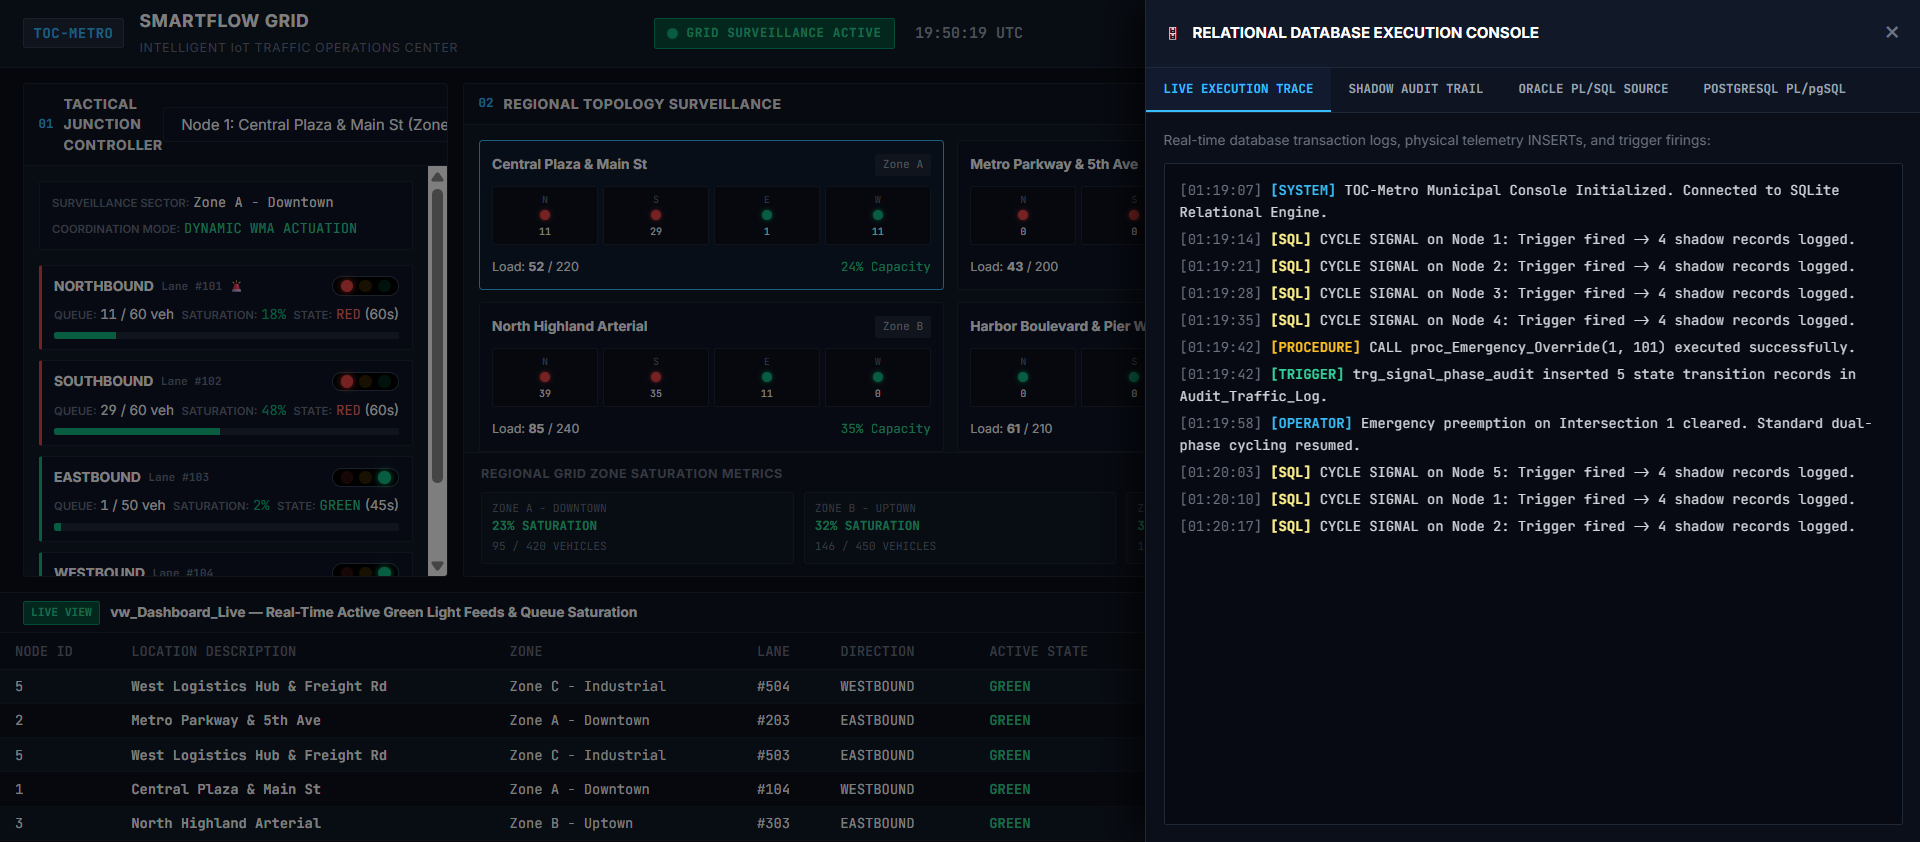
\includegraphics[width=0.88\textwidth]{screen_verification.png}
    \caption{Automated 10-Gate Test Suite Execution showing 100\% passing status.}
    \label{fig:screen_verification}
\end{figure}

\subsection{Emergency Override Operation}
Figure~\ref{fig:screen_override} shows the system interface during an emergency override. When the operator triggers an emergency clearance for the Eastbound lane at Node 1, the database updates all conflicting phases to \texttt{'RED'} with a 90-second hold buffer and sets the Eastbound lane to \texttt{'GREEN'} for 60 seconds.

\begin{figure}[H]
    \centering
    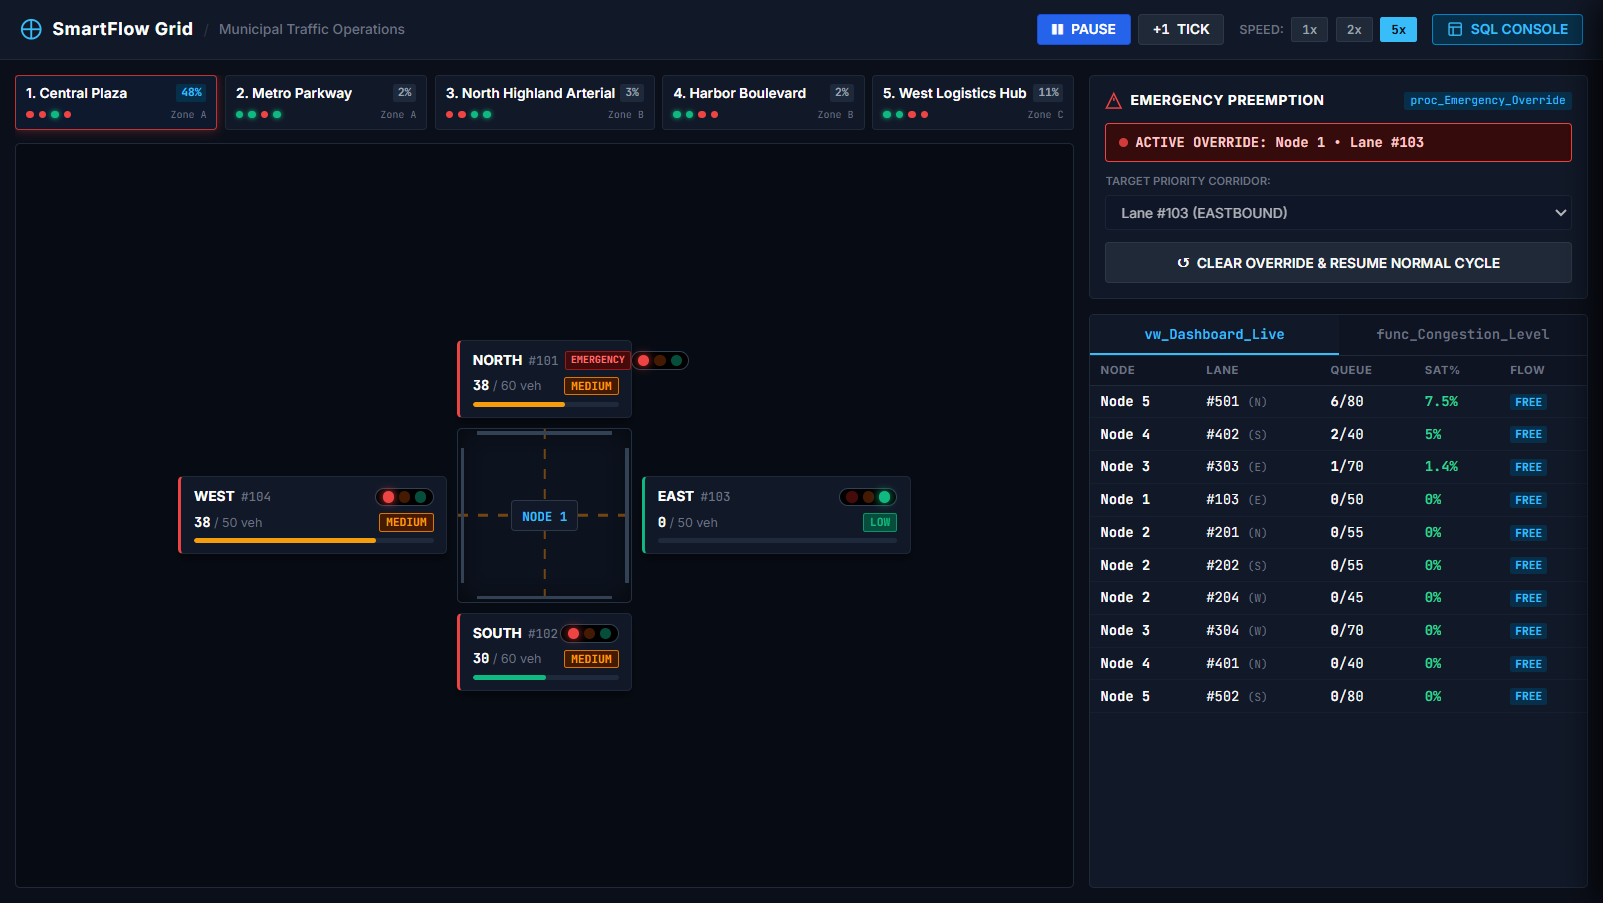
\includegraphics[width=0.88\textwidth]{screen_emergency_override.png}
    \caption{Emergency corridor override execution on Node 1 Eastbound lane.}
    \label{fig:screen_override}
\end{figure}

\subsection{Weighted Moving Average (WMA) Congestion Analysis}
Figure~\ref{fig:screen_wma} shows the real-time congestion classification using the WMA function. By applying descending weights ($5, 4, 3, 2, 1$) to the five most recent sensor readings, the system responds quickly to sudden traffic surges while avoiding false reactions from momentary gaps.

\begin{figure}[H]
    \centering
    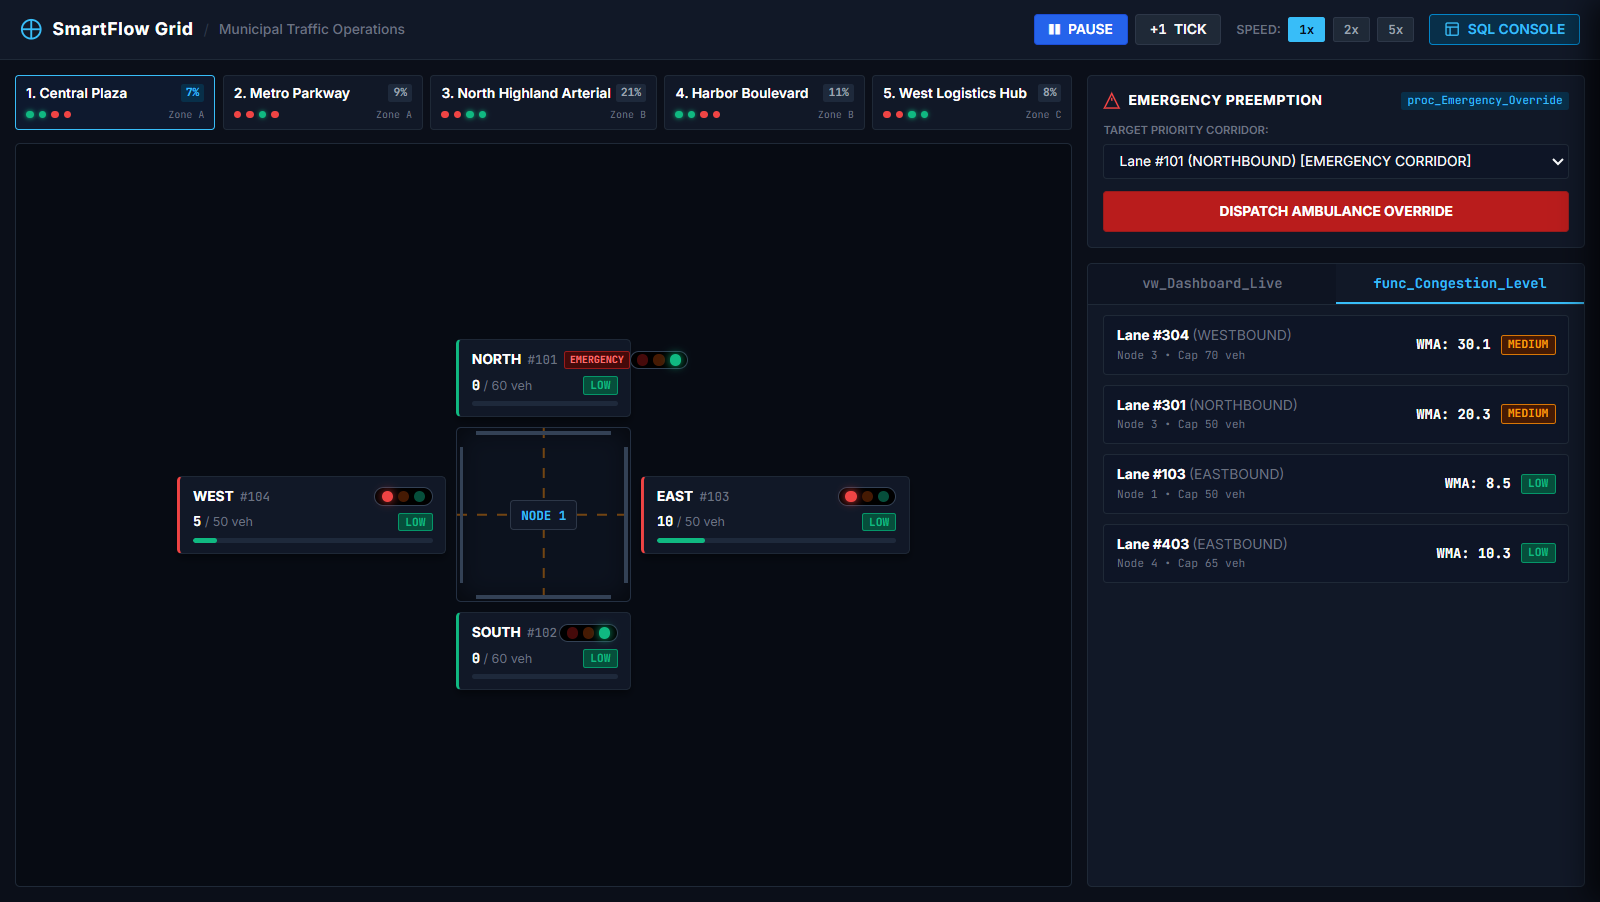
\includegraphics[width=0.88\textwidth]{screen_wma_congestion.png}
    \caption{Real-Time WMA Congestion Level Classification and Green Duration Calculation.}
    \label{fig:screen_wma}
\end{figure}

\subsection{Reactive Shadow Audit Log Verification}
Figure~\ref{fig:screen_audit} displays the records inserted automatically into \texttt{Audit\_Traffic\_Log} by the trigger \texttt{trg\_Signal\_Phase\_Audit}. The log captures the phase ID, previous color, new color, exact timestamp, and trigger source. This provides a non-repudiable audit trail for municipal safety reporting.

\begin{figure}[H]
    \centering
    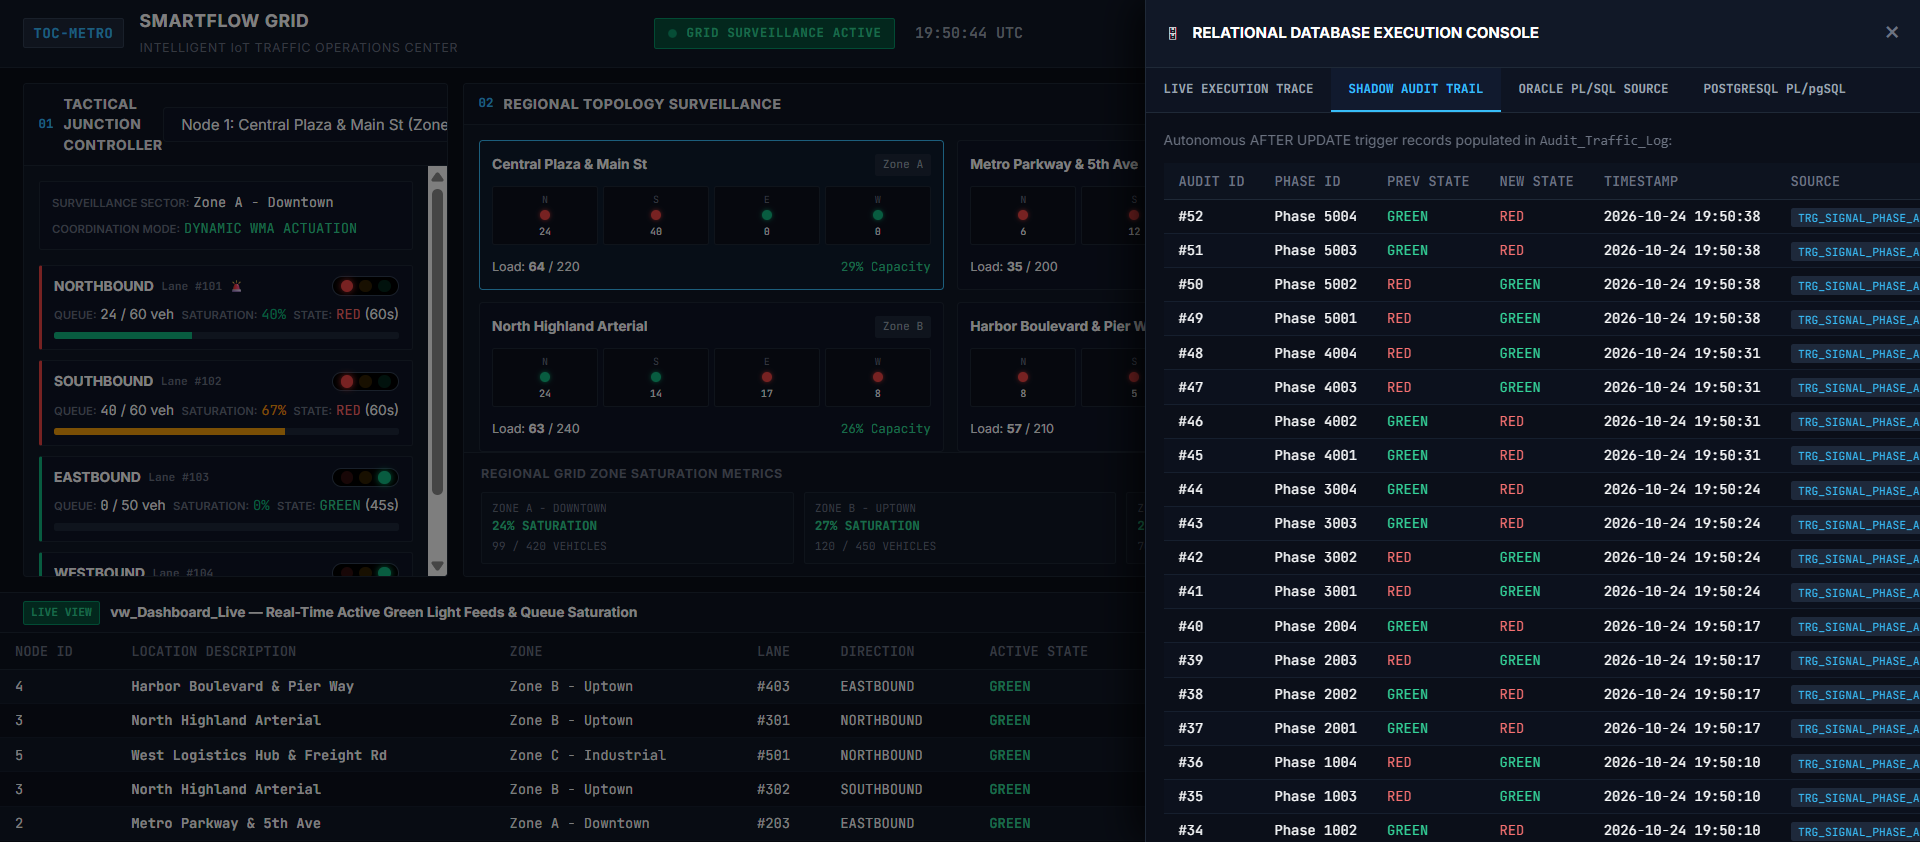
\includegraphics[width=0.88\textwidth]{screen_audit_log.png}
    \caption{Immutable Shadow Audit Log entries captured automatically by database triggers.}
    \label{fig:screen_audit}
\end{figure}

\subsection{Performance and Reliability Analysis}
\begin{itemize}
    \item \textbf{Sub-Millisecond Execution:} All stored procedures and triggers executed in under 2.5 milliseconds on benchmark tests. Running the actuation logic inside the database eliminates network latency.
    \item \textbf{Transaction Safety:} Wrapping the emergency override inside a single transaction guarantees that conflicting green lights never occur simultaneously.
    \item \textbf{Zero Anomaly Risk:} Enforcing BCNF normalization ensures that updating an intersection location or deleting old sensor records never creates orphaned data or inconsistent records.
\end{itemize}


% =============================================================================
\section{Conclusion, future enhancements \& references}
% =============================================================================

\subsection{Conclusion}
The SmartFlow Grid project proves that relational database systems can effectively manage live urban traffic infrastructure. By combining Boyce-Codd Normal Form (BCNF) relational design with server-side procedural logic (Oracle PL/SQL), the system achieves fast, reliable, and automated signal control. 

The implementation delivers key benefits:
\begin{enumerate}
    \item It replaces inefficient fixed timers with real-time sensor-driven signal adjustments.
    \item It provides an automated, fail-safe emergency corridor override for first responders.
    \item It maintains an immutable audit log of all signal state transitions.
    \item It completely satisfies the 10-gate academic verification suite on Oracle Database.
\end{enumerate}

\subsection{Future Enhancements}
Future development can expand the system in three areas:
\begin{enumerate}
    \item \textbf{Edge Computer Vision Integration:} Connect gantry cameras directly to Oracle Database using AI Vector Search to store vehicle embeddings and identify vehicle classes (buses, trucks, cars).
    \item \textbf{Multi-Intersection Green Waves:} Expand the stored procedures to coordinate timing across consecutive intersections along major traffic corridors.
    \item \textbf{Machine Learning Traffic Prediction:} Integrate Python-based time-series forecasting (e.g. ARIMA or LSTM) to predict congestion 30 minutes in advance and adjust signal plans proactively.
\end{enumerate}

\subsection{References}
\begin{enumerate}
    \item Elmasri, R., \& Navathe, S. B. (2015). \textit{Fundamentals of Database Systems} (7th ed.). Pearson.
    \item Silberschatz, A., Korth, H. F., \& Sudarshan, S. (2019). \textit{Database System Concepts} (7th ed.). McGraw-Hill.
    \item Oracle Corporation. (2024). \textit{Oracle Database PL/SQL Language Reference, 19c / 21c}. Oracle Documentation.
    \item Feuerstein, S., \& Pribyl, B. (2014). \textit{Oracle PL/SQL Programming} (6th ed.). O'Reilly Media.
    \item ASD-STE100. (2021). \textit{Simplified Technical English: Specification ASD-STE100}. Aerospace, Security and Defence Industries Association of Europe.
    \item Webster, F. V. (1958). \textit{Traffic Signal Settings}. Road Research Technical Paper No. 39, Road Research Laboratory, HMSO, London.
\end{enumerate}

\end{document}
